\chapter{IMPLEMENTATION DETAILS}
\section{Hardware Components}
\subsection{EEG Electrodes}
The basis for operation of EEG electrodes is based on biopotentials. The neural activity within the brain creates electrical potentials due to ions flowing through the membranes of the neurons. These potentials travel across the brain tissue and then to the scalp and skull, creating voltages.

In the experiment, EEG electrodes are placed on the scalp using the international 10-20 system. In the process, a differential method is applied where the voltage potential between the active electrode and the reference electrode is measured. Ground electrode is also used to stabilize the signal.

Blinking of eyes creates high-amplitude and low-frequency signals which are considered electrical artifacts. This is due to the fact that blinking causes eye muscles to contract.

\subsection{Instrumentation Amplifier (AD620)}
AD620 is a high precision instrumentation amplifier which is designed to amplify weak biomedical signals. Due to the nature of the signals generated by the brain, they are very weak and cannot be processed directly.

AD620 achieves amplification by amplifying the difference of two input signals and rejecting any common signal in the two input signals (common mode noise). This feature allows it to reject noise from mains, body movements, and the surrounding environment.
Gain in AD620 can be controlled through an external resistor.

\begin{figure}[H]
	\centering
	
\includegraphics[width = 14.5cm, height=6.5cm]{src/images/figures/instrumentation.png}
	\caption{Instrumentation Amplifier}
	\label{instrumentation}
\end{figure}


\subsection{High Pass Filter}
After instrumentation amplifier, the signals are sent to a highpass filter to remove DC components. This is done in two separate stages: filtering and amplification so that the DC components do not get amplified in the filtering stage.

In the filtering stage, there is unity gain and only high-pass filtering action is performed. The cutoff frequency is:
\[
f_c = \frac{1}{2\pi R_1 C_4}
\]
Substituting the values:
\[
f_c = \frac{1}{2\pi \cdot 3.3\,\text{k}\Omega \cdot 47\,\mu\text{F}} = 1.02\,\text{Hz}
\]

After that, we have a gain stage with gain:
\[
A_v = -\frac{R_4}{R_3}
\]
Substituting the values:
\[
A_v = -\frac{220\,\text{k}\Omega}{5\,\text{k}\Omega} = -44
\]

\begin{figure}[H]
	\centering
	
\includegraphics[width = 14.5cm, height=6.5cm]{src/images/figures/highpass.png}
	\caption{High Pass Filter}
	\label{highpass_filter}
\end{figure}

A small capacitor \(C_5 = 1\,\text{nF}\) is used in this stage, which is important in ensuring the stability of the circuit. It makes sure that there will be no high-frequency noise that can affect the signal and cause oscillation or vibration in the circuit. It can be considered as a kind of shock absorber to keep the signal steady all the time.

\subsection{Signal Amplification}
The first major problem in our project is that brain signals have very low strength. They are usually measured in microvolts, which means they are very tiny.

To make sure that these signals will be readable by a computer, we will use an instrument known as the AD620 Instrumentation Amplifier. Our choice of instrumentation amplifier is because it has the ability to eliminate any common mode noise such as electrical interference from wire and power sources. While other amplifiers add noise to the original signal, the ad620 is a much better option for our purpose.

As for the signal strength needed, we need to control the level of amplification, which is called gain (G).

In AD620, gain is controlled through only one resistor called Rg, connecting Pin 1 and Pin 8.
The formula is:
\[
G = \frac{49.4\,\text{k}\Omega}{R_g} + 1
\]

We decided to use a gain of 16.

Resistor calculation for gain:
\[
G = 16
\]

\[
16 = \frac{49.4}{R_g} + 1
\]

\[
16 - 1 = \frac{49.4}{R_g}
\]

\[
15 = \frac{49.4}{R_g}
\]

\[
R_g = \frac{49.4}{15}
\]

\[
R_g \approx 3.29\,\text{k}\Omega
\]

Since \(3.3\,\text{k}\Omega\) is a standard resistor value, we used \(3.3\,\text{k}\Omega\).

Since we do not apply high gain to boost the signal because it also contains a DC offset that is an unwanted constant voltage that offsets the AC signal. If we apply high gain at the early stages, then it will be large and may lead to saturation where the amplifier cannot accommodate the input anymore and clips the signal. So, we make sure that the initial gain is kept low.

Furthermore, we employ a Driven Right Leg technique, which involves averaging the measured signal and returning a small part of the averaged signal back to the body. The benefit of using this technique is that it helps reduce the common mode noise and interference that may affect the signal quality. Other than reducing noise, the driven right leg helps stabilize the body's reference point for safety purposes. Therefore, the final signal is very clean and free from noise and distortions.

\subsection{Analog Signal Conditioning Using Band Pass Filter}
The analog signal conditioning in the current project is performed using a band pass filter circuit, which serves as an all-in-one solution to the problems of high pass filtering, low pass filtering and rejection of power line interference. The use of a single band pass filter allows to filter out all undesired components and only leave the signal of interest.

The lower cut off frequency of the band pass filter serves as a means of blocking any DC offsets, as well as low frequency components resulting from electrode polarization and head movement. These components carry no useful information about the EEG signal and may impede its further amplification and digitization.

On the other hand, the higher cut off frequency of the band pass filter prevents high frequency noise from entering the system, such as EMG noise produced by muscles of the face and scalp, as well as electromagnetic interference. In order to isolate the brain activity, it is enough to restrict the higher end of the frequency range at 40 Hz.

Moreover, it should be noted that the current design includes a band pass filter, which rejects the component at 50 Hz, thus minimizing the effects of power line interference in the system.

The transfer function is shown below and describes the behavior of the output signal. Transfer function was obtained using nodal analysis, which is a common approach for designing active filters \cite{carter_opamp}. Following is the transfer function of the first stage.

Transfer function first stage:
\begin{equation}
	H_1(s)=\frac{V_o(s)}{V_{in}(s)}
	=\frac{-R_1 C_1\,s}{R_1R_2C_1C_2\,s^2+R_2(C_1+C_2)\,s+1}
\end{equation}

This stage begins removing unwanted signals and keeps the useful brain wave range.


\begin{equation}
	H_1(s)=\frac{-0.03728\,s}{8.0401776\times10^{-5}\,s^2+0.0059487\,s+1}
\end{equation}

\begin{figure}[H]
	\centering
	
\includegraphics[width = 10cm, height=3.5cm]{src/images/figures/filter_first.png}
	\caption{$1^{\text{st}}$ stage band-pass filter}
	\label{filter_first}
\end{figure}

Transfer function second stage:\newline
In this stage, the filter becomes stronger and more accurate. It removes even more unwanted noise using different resistors and capacitors.

\begin{equation}
	H_2(s)=\frac{V_o(s)}{V_{in}(s)}
	=\frac{-R_3 C_3 R_7 \, s}
	{R_3R_4R_7C_3C_4\,s^2+R_4R_7(C_3+C_4)\,s+(R_4+R_7)}
\end{equation}

\begin{figure}[H]
	\centering
	
\includegraphics[width = 10cm, height=3.8cm]{src/images/figures/filter_second.png}
	\caption{$2^{\text{nd}}$stage band-pass filter}
	\label{filter_second}
\end{figure}

\begin{equation}
	H_2(s)=\frac{-1.673\,s}{4.107\,s^2+254.317\,s+87900}
\end{equation}

Transfer function third stage:\newline
This is the final cleanup stage. It works like Stage 2 but uses slightly different values to fine tune the signal. This stage ensures the signal is very clean and ready for use.

\begin{equation}
	H_3(s)=\frac{V_o(s)}{V_{in}(s)}
	=\frac{-R_5 C_5 R_8\,s}
	{R_5R_6R_8C_5C_6\,s^2+R_6R_8(C_5+C_6)\,s+(R_6+R_8)}
\end{equation}

\begin{figure}[H]
	\centering
	
\includegraphics[width = 10cm, height=3.8cm]{src/images/figures/filter_third.png}
	\caption{$3^{\text{rd}}$stage band-pass filter}
	\label{filter_third}
\end{figure}

\begin{equation}
	H_3(s)=\frac{-3.40331\,s}{14.4350344\,s^2+516.864\,s+103300}
\end{equation}

Final transfer function:
\begin{equation}
	H(s)=H_1(s)H_2(s)H_3(s)
\end{equation}

\begin{align}
	H(s) &=
	\frac{(-0.03728s)(-1.673s)(-3.40331s)}
	{(8.040\times10^{-5}s^2+0.0059487s+1)
		(4.107s^2+254.317s+87900)} \notag \\
	&\quad \times
	\frac{1}
	{(14.435s^2+516.864s+103300)}
\end{align}

\begin{figure}[H]
	\centering
	
\includegraphics[width = 14.5cm, height=6.5cm]{src/images/figures/three_stage.png}
	\caption{Three-stage $6^{\text{th}}$-order band-pass filter}
	\label{three_stage}
\end{figure}


\subsection{Arduino Microcontroller (ADC \& Control Unit)}
The role of the Arduino is to serve as an interface between the analog EEG hardware and the computer. This is because the Arduino board comes with an integrated analog to digital converter (ADC) that converts the conditioned analog signals into digital information.

The ADC measures the input voltage periodically and translates it into a numeric value depending on the reference voltage and ADC resolution (normally 10 bits). The resulting digital signal can be manipulated through software. Subsequent to this conversion, the Arduino transfers the information to the computer using the USB serial connection (internally uses the UART protocol).

\subsection{Timer1 - Arduino}
The Timer1 of arduino is configured in CTC mode to generate interrupts at a rate of 1024 Hz. This allows the Arduino to sample the analog input at at desired intervals and independant of the main program. The configuration details are:

\begin{itemize}
	\item {Timer:} Timer1 (16-bit)
	\item {Mode:} CTC (Clear Timer on Compare Match)
	\item {Prescaler:} 1
	\item {Compare Register (OCR1A):} 31249
	\item {Interrupt Frequency:} 
	\[
	f_\text{interrupt} = \frac{f_\text{CPU}}{(OCR1A + 1) \times \text{Prescaler}} 
	= \frac{16\,\text{MHz}}{31249 \times 1} = 512~\text{Hz}
	\]
\end{itemize}

\noindent The ISR reads the analog input and stores it in a double buffer for further processing:

\subsection{Interconnection of Hardware Components}
All hardware devices are interconnected to develop an effective EEG-based BCI system. Signals from the brain along with eye blink activity are recorded using EEG electrodes and are amplified using the AD620 instrumentation amplifier. Amplified signals are filtered using the bandpass filter in order to eliminate the noise.

The filtered signal is then digitized using the ADC feature of the Arduino microcontroller. The digital signal is transferred to MATLAB using the serial port. Signal processing is done in MATLAB using FFT and time domain analysis for the detection of eye blinks and brain waves activity. According to the set threshold values, control commands are generated using rules and are mapped to simple text entry device.

This hardware-software combination proves to be an effective and economical example of BCI system.

\section{Software Components}
\subsection{Arduino Firmware}
The Arduino firmware serves as the data acquisition and communication interface of the project. Its main purpose is to continuously acquire the filtered EEG signal from the analog input pin via the built-in Analog to Digital Converter (ADC) of the board and send it to the computer.

The ADC of the Arduino digitizes the incoming analog EEG signal using the board's reference voltage and ADC resolution. In the present project, the amplified and filtered EEG signal falls within the safe operating limits of the Arduino's ADC. The firmware is written in such a way as to acquire the signal at a fixed and constant sampling frequency to enable frequency domain analysis using FFT in MATLAB.

The sampling period of the ADC can be achieved through the use of a timer or delay function in the firmware code. The acquired samples are transmitted in real-time to the computer via the USB serial communication protocol, which uses the UART interface. The baud rate of the USB serial connection is chosen to enable lossless real-time data transfer.

The Arduino firmware does not do any complex signal processing. It is only responsible for data acquisition and real time transmission of the acquired data. All other processing tasks are done using MATLAB.
Functions in the Project:
\begin{itemize}
	\item To read analog EEG signal using Arduino ADC
	\item Maintain constant sampling frequency
	\item Convert analog voltage into corresponding digital values
	\item Send the digital data to MATLAB via USB serial link
\end{itemize}


\subsection{MATPLOTLIB}
Python is used as the platform for signal processing, analysis, and visualization in the proposed project. Real time EEG data sent via serial port from Arduino microcontroller is processed in Python using digital signal processing techniques. Various Python libraries like NumPy, SciPy and Matplotlib are used for computing, frequency analysis and graphical visualization respectively.

Initially, the acquired EEG samples are plotted in the time domain using the Matplotlib library. The eye blink events can be identified as high amplitude peaks in the time domain waveform. The Python program continuously checks the amplitude value of the received signal and uses a threshold-based algorithm to detect eye blinks in real time.

The frequency analysis of brain waves requires the signal to be segmented into short time segments of equal duration. Each time segment is subjected to a Hann window before performing the Fast Fourier Transform (FFT) in order to reduce spectral leakage. The NumPy and SciPy libraries are used to compute FFT in order to convert the EEG signal from time domain to frequency domain.

In this experiment, we are interested in analyzing the beta waves which lie in the frequency band between 12 Hz to 30 Hz. The Python program computes the spectral power in this frequency band and compares it with the pre-defined threshold to estimate the user's mental state like relaxed or focused.

Eye blink detection and beta wave detection are considered as the features in the project. Eye blink detection serves as a control/selection function while beta wave detection serves as a decision factor. Rule based decision algorithm generates command to the text selection interface based on the detections mentioned above. The results and plots are displayed using Matplotlib library showing a human-computer interaction system driven by brain signals.


\section{Calibration Process of Each Module}
\subsection{EEG Electrode Calibration}
\begin{itemize}
	\item Skin preparation is carried out to minimize impedance between electrodes
	\item Electrodes are tightly fixed to minimize movement and provide stable contact
	\item Baseline brain waves are collected to confirm the availability of the EEG signal
\end{itemize}

\subsection{Amplifier Calibration}
\begin{itemize}
	\item The gain of AD620 amplifier is set using external resistors
	\item Output response is evaluated using low amplitude input signals
	\item Offset voltage is checked to avoid saturation of signals
\end{itemize}

\subsection{Filter Calibration}
\begin{itemize}
	\item High and low pass cutoff frequencies are checked
	\item Filter frequency response is measured using signal generators
\end{itemize}

\subsection{ADC Calibration}
\begin{itemize}
	\item Reference voltage for Arduino ADC is confirmed
	\item Input signal range is checked to avoid clipping
	\item Sampling frequency is evaluated for accurate FFT
\end{itemize}




\section{Interfacing Technicalities and Protocols}
\subsection{EEG Electrodes to Amplifier Interface}
The interfacing of the EEG electrodes with the instrumentation amplifier occurs through the use of differential connection techniques. Here, two active electrodes are employed to detect the voltage difference produced by brain activity with a reference electrode for comparison purposes. The ground electrode acts as the common reference point of the system where it is connected to the body of the subject under study. This is necessary since EEG signals are very small in magnitude and easily susceptible to interference.

Shielding of the wires connecting the electrodes to the amplifier inputs is done to prevent any form of electromagnetic interference from other electrical devices. Appropriate skin preparation and tight electrode attachment are critical in minimizing the electrode-skin impedance. This ensures that no distortion of the signal occurs. The differential connection technique enables the amplifier to accurately pick the EEG signals and artifacts caused by eye blinks.

\subsection{Amplifier to Filter Circuit Interface}
The output from the AD620 instrumentation amplifier is connected directly to the input of the analog filter circuit. Signal matching is vital at this point since the amplified signal must stay within the operational range of the filter circuit components. Gain adjustment of the amplifier is carried out to make sure that the amplified signal is large enough for filtering purposes without saturating the filter circuitry.

Grounding techniques are applied to eliminate possible ground loops which could lead to more noise and system instability. Both amplifier and filter circuits have a common ground to ensure signal integrity. Connecting the amplifier output directly to the filter input makes sure that signal flow is uninterrupted throughout this part of the process and undesired frequencies are eliminated.

\subsection{Filter to Arduino Interface}
After the analog conditioning of the signal, the filtered EEG signal will be connected to the Arduino microcontroller using an analog input pin on the microcontroller. Because the analog to digital converter (ADC) used in the microcontroller cannot take input voltages greater than 5 volts, it is ensured that the filtered output voltage stays below this maximum level.

The filtered output signal corresponds to the clean EEG signal which contains brain activities and eye blink events. This signal is fed to the analog input pin of the microcontroller where it is sampled at equal intervals. The ground connection between the filter circuit and the microcontroller remains common for both of them.
\subsection{Fast Fourier Transform}
FFT is used to analyze the frequency components of the signal.The pseudocoe for the implementation of FFT is given below:

\begin{algorithm}[H]
	\caption{Cooley-Tukey FFT}
	\label{alg:fft}
	\begin{algorithmic}[1]
		\Require $x[0..N-1]$: sequence of sample, $N$ a power of 2
		\Ensure $X[0..N-1]$: discrete Fourier transform of $x$
		\If{$N = 1$}
		\State $X[0] \gets x[0]$
		\Else
		\State $x_\text{even} \gets x[0], x[2], \dots, x[N-2]$
		\State $x_\text{odd} \gets x[1], x[3], \dots, x[N-1]$
		\State $X_\text{even} \gets \text{FFT}(x_\text{even})$
		\State $X_\text{odd} \gets \text{FFT}(x_\text{odd})$
		\For{$k = 0$ to $N/2 - 1$}
		\State $t \gets X_\text{odd}[k] \cdot e^{-2 \pi i k / N}$
		\State $X[k] \gets X_\text{even}[k] + t$
		\State $X[k + N/2] \gets X_\text{even}[k] - t$
		\EndFor
		\EndIf
		\State \Return $X$
	\end{algorithmic}
\end{algorithm}

\textbf{Bit Reversal}\newline
The bit reversal technique is a preprocessing step used in the Cooley-Tukey Fast Fourier Transform (FFT) to enable in place computation and reduce memory usage. In the FFT, the input sequence is recursively divided into even and odd indexed elements. This recursion can consume extra memory due to multiple temporary arrays.

We can reorder the sample sequence to perform the computation with low memory cost using bit reversal by reversing bits. For our use 1 byte memory is more than enough for bit reversal so we have put in pre defined array as 64 sized array is enough for this computation. After reordering, the FFT algorithm can operate iteratively and in place, eliminating the need for recursive subarrays. This reduces memory overhead, improves cache efficiency, and allows the FFT to maintain its computational complexity of $N \log N$.

An N point signal is decomposed into N signals each containing a single point.
Each stage uses an interlace decomposition, separating the even and odd numbered samples.
\begin{figure}[H]
	\centering
	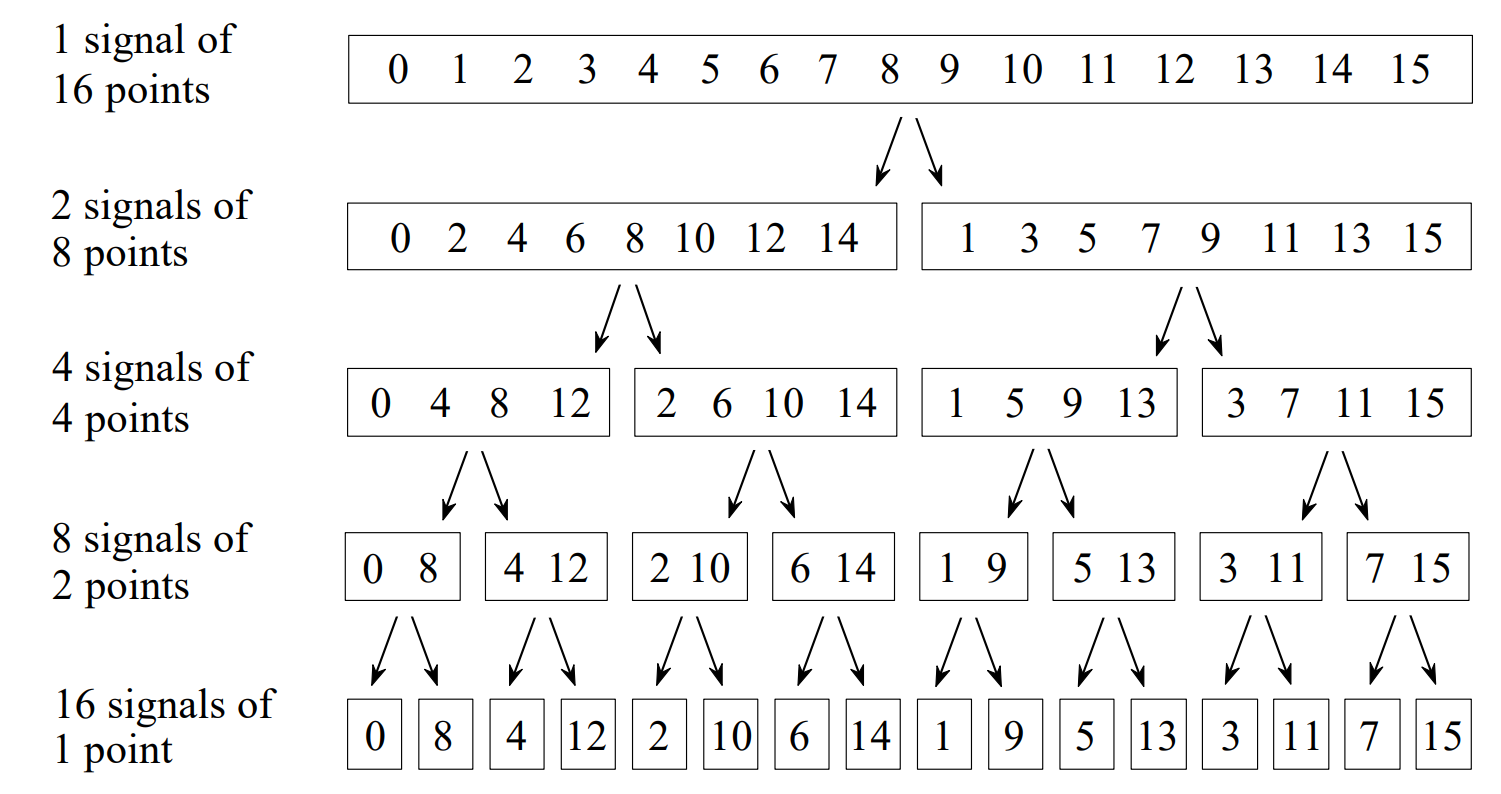
\includegraphics[width = \textwidth, height=7cm]{src/images/figures/odd_even.png}
	\caption{The FFT sample decomposition. \cite{smith1999dsp}
	}
	\label{odd_even}
\end{figure}

\begin{table}[H]
	\centering
	\caption{Bit-reversal permutation for $N=8$ FFT}
	\label{tab:bitreversal}
	\begin{tabular}{c c c c}
		\hline
		\textbf{Original Index} & \textbf{Binary} & \textbf{Reversed Binary} & \textbf{Bit-Reversed} \\ 
		\hline  % thinner line between header and data
		0 & 000 & 000 & 0 \\
		1 & 001 & 100 & 4 \\
		2 & 010 & 010 & 2 \\
		3 & 011 & 110 & 6 \\
		4 & 100 & 001 & 1 \\
		5 & 101 & 101 & 5 \\
		6 & 110 & 011 & 3 \\
		7 & 111 & 111 & 7 \\
		\hline
	\end{tabular}
\end{table}

\subsection{Arduino to MATLAB Communication Interface}
Data transfer between the Arduino and the MATLAB is performed via USB-based serial communication, where the internal protocol used by the USB-based serial communication is UART (Universal Asynchronous Receiver Transmitter). Arduino sends the digitized data from the EEG sample to the computer in the form of serial packets.

Baud rate for the serial communication is chosen appropriately such that there is no loss or corruption of the transmitted data due to the high speed of transfer. The MATLAB opens a serial port to receive the data packet, synchronizes with the Arduino, and performs real-time processing on the received samples.



